
\subsection{First Day TOPP Value Comparison} \label{ss:day1} %first day comparison

\begin{figure}
    \centering
    \includegraphics[width=\textwidth]{img/first_day_values}
    \vspace{0mm}
    \caption{MCM v3.2 first day TOPP values and corresponding values in each mechanism.}
    \vspace{-4mm}
    \label{f:first_day}
\end{figure}

\begin{figure}
    \centering
    \includegraphics[width=\textwidth]{img/Ox_tagged_budget_overlay_all_mechanisms}
    \vspace{0mm}
    \caption{\ce{O_x} production budgets allocated to individual VOCs.}
    \vspace{-4mm}
    \label{f:Ox_tagged_budgets}
\end{figure}

The first day TOPP values calculated from each mechanism are compared to those obtained with the MCM v3.{2} in Figure \ref{f:first_day}. 
The reduced mechanisms generally match the \mbox{MCM v3.2} first day TOPP values. 
However TOPP values resulting from aromatic VOC degradation are lower in reduced mechanisms.

Aromatic chemistry is difficult to represent in chemical mechanisms as many products, their yields and reactions are not known or subject to uncertainties \citep{Vereecken:2012}. 
Thus, greater variation is expected between aromatic VOC TOPP values.
The largest discrepancies are the zero TOPP values of toluene and m-xylene in RACM. 
This is unrealistic as aromatic VOCs contribute significantly to \ce{O_x} production \citep{Derwent:1998}. 
Section \ref{sss:aromatic} outlines the responsible chemistry.

The $2$-methylpropene first day TOPP values in RACM, RACM2, CBM-IV and CB05 indicate that its degradation is treated differently to the MCM v3.2. 
The variation between RACM, RACM2 and MCM v3.2 arises from differences in $2$-methylpropene ozonolysis rate constants.
In RACM and RACM2 this is a weighted mean of all VOC ozonolysis rate constants represented as OLI \citep{Stockwell:1997, Goliff:2013} and is an order of magnitude faster than MCM v3.2 despite a common source (IUPAC).
The resulting increased radical production leads to more \ce{O_x} production than in the MCM v3.2.

In CBM-IV, $2$-methylpropene is represented by the mechanism species ALD2 \citep{Hogo:1989}, which is a surrogate for aldehydes with more than one carbon atom. 
ALD2 reacts very quickly with OH forming \ce{CH3CO3}, leading to \ce{O_x} production. 
Furthermore, ALD2 photolysis promotes radical and in turn \ce{O_x} production. 
This is not a degradation pathway for $2$-methylpropene in any other mechanism. 
The choice of $2$-methylpropene representation gives rise to higher \ce{O_x} production than in the MCM v3.2.

$2$-methylpropene representation was updated in CB05 to \mbox{FORM + $3$ PAR}, where FORM represents formaldehyde and PAR the paraffin \ce{C-C} bond \citep{Yarwood:2005}. 
The initial formaldehyde oxidation reactions are similar to ALD2 whilst PAR is a slow reacting species. 
This slows down the \ce{O_x} production resulting in lower \ce{O_x} production than in the MCM v3.2.

Many CBM-IV and CB05 first day TOPP values are lower than those of the \mbox{MCM v3.2}. 
Lower \ce{O_x} production in CBM-IV and CB05 compared to MCM v3.2 is responsible.
This is shown in \mbox{Figure \ref{f:Ox_tagged_budgets}} where \ce{O_x} production is allocated to parent VOCs in each mechanism.
Lower \ce{O3} levels using CBM-IV and CB05 compared to other mechanisms have also been noted in previous modelling studies such as \citet{Luecken:2008, Emmerson:2009} and \citet{Saylor:2012}.

\subsection{TOPP Value Time Series} \label{ss:profiles} %TOPP time series of all species

\begin{figure}
    \centering
    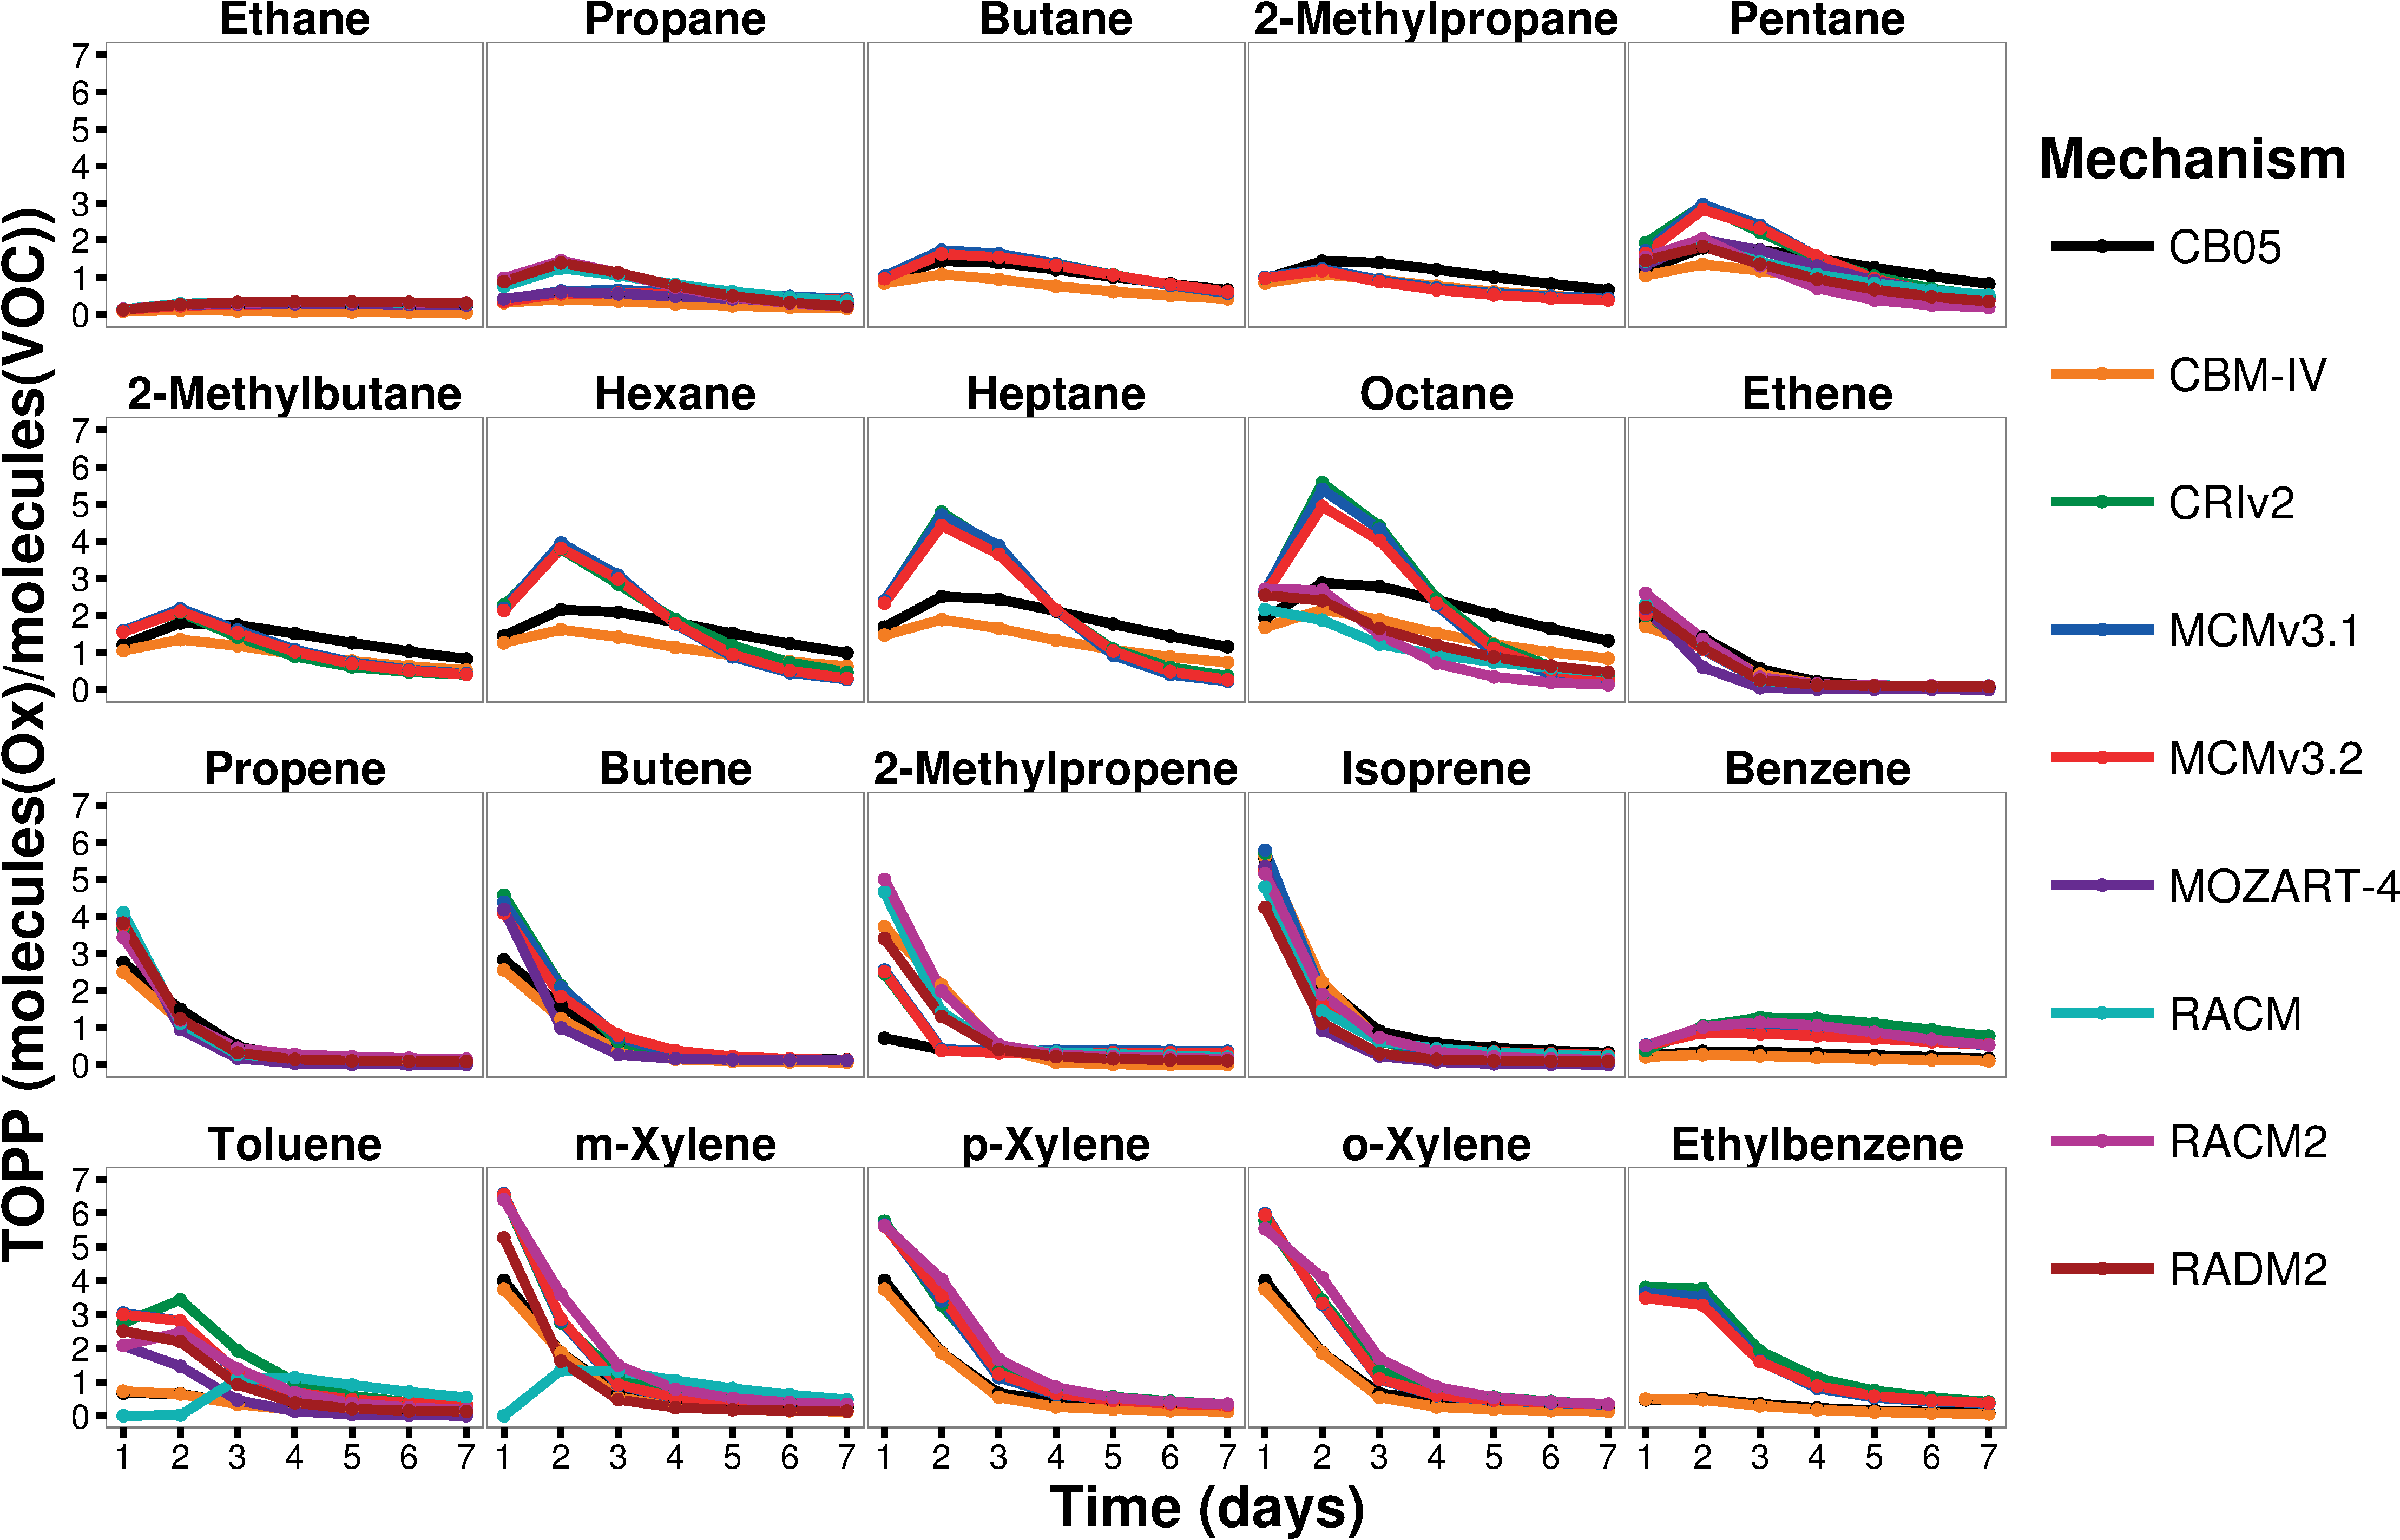
\includegraphics[width=\textwidth]{img/TOPP_daily_values_all_species}
    \vspace{0mm}
    \caption{TOPP value time series for all NMVOCs obtained with each mechanism.}
    \vspace{-4mm}
    \label{f:TOPP_dailies}
\end{figure}

NMVOC daily TOPP value time series are presented in \mbox{Figure \ref{f:TOPP_dailies}}. 
NMVOCs, such as ethene, whose degradation is described using dedicated mechanism species show similar time-dependent \ce{O_x} production.
Higher variability emerges between the time series of those NMVOCs represented by lumped mechanism species, such as pentane.

\ce{O_x} production from alkane degradation has a second day maximum increasing with carbon number in CRI v2 and both MCM mechanisms.
Octane degradation in RADM2, RACM and RACM2 is the exception as it is broken down into smaller sized fragments quicker than the MCM v3.2.
This analysis is outlined in Section \ref{s:detailed_results} and octane results are found in the supplement.

Aromatic VOC \ce{O_x} production has the most variability between mechanisms. 
In particular, zero \ce{O_x} production for toluene and m-xylene when using RACM.

\ce{O_x} production from toluene degradation in CBM-IV and CB05 is much lower than in the MCM v3.2.
This impacts ethylbenzene \ce{O_x} production as it is represented as \mbox{TOL + PAR}. 
Toluene degradation in RACM, CBM-IV and CB05 is summarised in Section \ref{sss:aromatic}.  

\subsubsection{Toluene Degradation in RACM, CBM-IV and CB05} \label{sss:aromatic}

\begin{figure}
    \centering
    \includegraphics[width=\textwidth]{img/TOL_Ox_intermediates}
    \vspace{0mm}
    \caption{Day-time \ce{O_x} production and consumption budgets from toluene degradation in \mbox{(a) MCM v3.2}, (b) RACM, (c) CBM-IV and (d) CB05.}
    \vspace{-4mm}
    \label{f:toluene_Ox}
\end{figure}

\ce{O_x} production and consumption day-time budgets from toluene degradation in \mbox{MCM v3.2}, RACM, CBM-IV and CB05 are depicted in Figure \ref{f:toluene_Ox}. 
The tagging approach allows attribution to the contributing organic reactions.

RACM chemistry results in net \ce{O_x} loss on the first two days in contrast to net \ce{O_x} production using the MCM v3.2.
This is due to several \ce{O_x}-consuming reactions in RACM not present in the MCM.
Cresol OH-adduct mechanism species ADDC ozonolysis contributes the most to \ce{O_x} loss.
A fast rate constant \mbox{($5 \times 10^{-11}$ cm$^3$ s$^{-1}$)} was assigned making it the main ADDC reaction pathway. 
This reaction was included due to improved cresol product yields when comparing RACM predictions with experimental data \citep{Stockwell:1997}.

Other mechanisms including cresol OH-adduct species do not include ozonolysis.
Including aromatic OH-adduct species ozonolysis in RACM results in non-representative \ce{O_x} production. 
This was updated in RACM2 and aromatic OH-adduct species ozonolysis are no longer included.

Cresol OH-oxidation is the highest contributor to both \ce{O_x} production and reactive carbon loss during CBM-IV and CB05 toluene degradation.
Reactive carbon loss leads to overall lower ability to produce \ce{O_x} during toluene degradation in CBM-IV and CB05.
Section \ref{s:detailed_results} details reactive carbon loss analysis and the supplement shows the reactions responsible for reactive carbon loss from toluene degradation.

\subsection{Radical Sources} \label{ss:radicals}

\begin{figure}
    \centering
    \includegraphics[width=\textwidth]{img/radical_production_analysis}
    \vspace{0mm}
    \caption{Net radical production day-time budgets for each mechanism. Net radical production calculated as the difference between radical and \ce{NO_x} yields. O1D represents the reaction of \ce{O(^1D)} with water vapour.}
    \vspace{-4mm}
    \label{f:radical_production} 
\end{figure} 

Maximum \ce{O_x} production was achieved by emitting the NO amount required to balance the radical source at each time step. 
Mechanism differences in radical production lead to different NO emissions.

Figure \ref{f:radical_production} depicts the day-time net radical production budgets in each mechanism allocated to the contributing reactions.
Reactions having net radical to \ce{NO_x} yield were determined for each mechanism and the rate was multiplied by this yield.

CBM-IV and CB05 have much higher net radical production on the first two days than any other mechanism.
Thus larger NO emissions are required for maximal \ce{O_x} production indicating that CBM-IV and CB05 represent \ce{NO_x}-sensitive chemistry.

CBM-IV was developed for the high-\ce{NO_x} conditions of urban and polluted regions \citep{Gery:1989}.
Hence, CBM-IV lacks low-\ce{NO_x} chemistry such as organic peroxide formation.
CB05 includes more oxygenated species so that organic peroxide chemistry is represented \citep{Yarwood:2005}.
However, CB05 net radical production is still significantly large.

The \ce{O(^1D)} and water vapour reaction is the main radical source in each mechanism.
Varying \ce{O3} levels in each mechanism leads to different \ce{O(^1D)} amounts as its main source is \ce{O3} photolysis.
Carbonyl, mainly HCHO, photolysis is the main radical source from organic chemistry.
Moreover, each mechanism has a similar contribution from HCHO photolysis.

Methyl glyoxal photolysis has a varying impact on net radical production in each mechanism.
\mbox{Section \ref{sss:mglyox}} describes methyl glyoxal production in all mechanisms and explains these differences.

Most reduced mechanisms lack sufficient carbonyl species to sustain radical production solely through carbonyl photolysis.
Initial VOC oxidation, NO--\ce{RO2} reactions and ozonolysis are used to further sustain radical production in less-explicit mechanisms.
Examples of non-photolysis radical sources are given in Table \ref{t:thermal_radicals}.

Mechanisms require different NO emissions to simulate \ce{NO_x}-VOC-sensitive conditions.
Thus, a constant NO source may lead to different atmospheric regimes being simulated depending on the mechanism.
This shall be investigated in future work.
{%
    \renewcommand{\arraystretch}{1.3}
    \begin{table}
        \centering
        \small
        \begin{tabular}{lP{3.0cm}P{2.5cm}P{2.5cm}}
            \hline \hline
            \textbf{Mechanism} & \textbf{VOC Oxidation} & \textbf{\ce{RO2 + NO}} & \textbf{Ozonolysis} \\ \hline \hline
            RADM2 & HC5 + OH & NO + TCO3 & \\ \hline
            \multirow{2}{*}{RACM2} & & & DCB + O3 \\
            & & & EPX + O3 \\ \hline
            \multirow{3}{*}{CBM-IV} & C2H4 + OH & C2O3 + NO & \\
            & CH4 + OH & & \\
            & OH + PAR & & \\ \hline
            \multirow{3}{*}{CB05} & C2H6 + OH & CXO3 + NO & \\
            & C2H4 + OH & & \\
            & OH + PAR & & \\ \hline \hline
        \end{tabular}
        \vspace{1mm}
        \caption{Non-photolysis radical producing reactions.}
        \vspace{-4mm}
        \label{t:thermal_radicals}
    \end{table}
}%

\subsubsection{Methyl Glyoxal Production} \label{sss:mglyox}

\begin{figure}
    \centering
    \includegraphics[width=\textwidth]{img/MGLY_VOC_allocated_production_rates}
    \vspace{0mm}
    \caption{Methyl glyoxal production budgets allocated to parent VOCs in each mechanism.}
    \vspace{-4mm}
    \label{f:mglyox_budgets} 
\end{figure} 

Methyl glyoxal is represented in each mechanism -- MGLYOX in both MCM versions, CARB6 in CRI v2, CH3COCHO in MOZART-4 and MGLY in RADM2, RACM, RACM2, CBM-IV and CB05.
NMVOC degradation is the only source and Figure \ref{f:mglyox_budgets} shows the individual sources in each mechanism.

Isoprene and aromatic VOC degradation are the main methyl glyoxal sources in all mechanisms except RADM2, RACM and RACM2.
In these mechanisms, pentane and propane degradation produce the most methyl glyoxal.
MOZART-4 pentane degradation also produces methyl glyoxal.
The supplement shows the pentane degradation reactions influencing the methyl glyoxal production budget.

Acetone degradation in low-\ce{NO_x} conditions produces methyl glyoxal through the acetone peroxy radical reaction with other \ce{RO2} \citep{Fu:2008}.
This is represented in both MCM versions and is a minor source as \ce{NO_x}-VOC-sensitive conditions are used.  
MOZART-4 also includes this chemistry but the rate constant is four times faster than the MCM v3.2, leading to higher MOZART-4 production.

The NO + KETP reaction, KETP is the ketone peroxy radical, produces additional methyl glyoxal under high-\ce{NO_x} conditions in RADM2, RACM and RACM2.
This additional pathway results in higher methyl glyoxal production from alkane degradation in these mechanisms.

Methyl glyoxal production from acetone degradation is not included in CBM-IV and CB05 as high-\ce{NO_x} conditions are assumed.
In CRI v2, the acetone peroxy radical (RN8O2) skips methyl glyoxal production altogether and immediately produces \ce{CH3CO3}.
